\section{Metric distances}

Vector spaces, equipped with some (weighted) $L_p$-norm, are not general enough to deal with the whole variety of feature types and distance functions needed for MM data. 

\paragraph*{Metric spaces}
A metric space $M = (U,d)$ is a pair, where:
$U$ is a domain of values, and $D$ is a distance function that, $\forall x,y,z \in U$, satisfies the metric axioms:
\begin{itemize}
    \item \textit{Positivity}: $D(x,y) \geq 0, D(x,y) = 0 \leftrightarrow x = y$.
    \item \textit{Symmetry}: $D(x,y) = D(y,x)$. 
    \item \textit{Triangle inequality}: $D(x,y) \leq D(x,z) + D(z,y)$. 
\end{itemize}
All the distance functions seen previously are metrics, and so are the (weighted) $L_p$-norms. 
Metric indexes only use the metric axioms to organize objects, and exploit the triangle inequality to prune the search space. 

\paragraph*{Shape matching}
Given two sets of points $S_1$ and $S_2$: 
\begin{figure}[H]
    \centering
    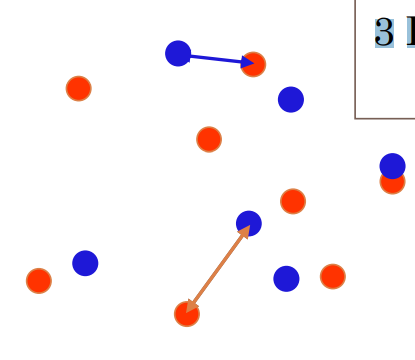
\includegraphics[width=0.5\linewidth]{images/hd.png}
\end{figure}
The Hausdorff distance is defined as follows:
\begin{enumerate}
    \item For all gray point of $S_1$ find the closest black point in $S_2$. 
        Let $h(S_1,S_2)$ be the maximum of such distances. 
    \item For all black point in $S_2$ find the closest gray point in $S_1$. 
        Let $h(S_2,S_1)$ be the maximum of such distances. 
    \item Compute the Hausdorff distance as: 
        \[\text{D}_{\text{Haus}}(S_1,S_2) = \max\{ h(S_1,S_2),h(S_2,S_1)\}\]
\end{enumerate}
This technique is useful for matching shapes. 

\paragraph*{Set similarity}
To compute the difference and the similarities between two sets $s_1$ and $s_2$, it is possible to use the function: 
\[D_{setdiff}(s_1,s_2)=\dfrac{\left\lvert s_1 - s_2 \right\rvert \left\lvert s_2 - s_1 \right\rvert }{\left\lvert s_1 \left\lvert +\right\rvert s_2 \right\rvert}\]

\paragraph*{Edit distance}
The edit distance is a common distance measure for strings, defined as the minimum number of characters that have to be inserted, deleted, or substituted to transform a string $s_1$ into another string $s_2$. 
\begin{example}
    Consider the following pairs: 
    \begin{enumerate}
        \item $\left\langle \text{ball},\text{bull} \right\rangle$.
        \item $\left\langle \text{balls},\text{bell} \right\rangle$.
        \item $\left\langle \text{rather},\text{alter} \right\rangle$.
    \end{enumerate}
    The corresponding edit distances are: 
    \begin{enumerate}
        \item $D_{\text{edit}}(\text{ball},\text{bull})=1$.
        \item $D_{\text{edit}}(\text{balls},\text{bell})=2$.
        \item $D_{\text{edit}}(\text{rather},\text{alter})=3$.
    \end{enumerate}
\end{example}
The edit distance is also used in genomic DB's to compare DNA sequences.
Thus, each DNA sequence is a string over the 4-letters alphabet of bases. 
\begin{example}
    Consider the pair $\left\langle \text{rather},\text{alter} \right\rangle$. 
    The edit distance can be computed with two matrices. 
    We initially define the cost matrix as follows: 
    \begin{table}[H]
        \centering
        \begin{tabular}{c|c|c|c|c|c|c|}
        \hline
        \multicolumn{1}{|c|}{\textbf{r}} & 1         & 1          & 1          & 1          & 1          & 0          \\ \hline
        \multicolumn{1}{|c|}{\textbf{e}} & 1         & 1          & 1          & 1          & 0          & 1          \\ \hline
        \multicolumn{1}{|c|}{\textbf{h}} & 1         & 1          & 1          & 0          & 1          & 1          \\ \hline
        \multicolumn{1}{|c|}{\textbf{t}} & 1         & 1          & 1          & 1          & 1          & 1          \\ \hline
        \multicolumn{1}{|c|}{\textbf{a}} & 1         & 0          & 1          & 1          & 1          & 1          \\ \hline
        \multicolumn{1}{|c|}{\textbf{r}} & 1         & 1          & 1          & 1          & 1          & 0          \\ \hline
        \multicolumn{1}{|c|}{$\uparrow$}& 0         & 1          & 1          & 1          & 1          & 1          \\ \hline
                                         & $\rightarrow$ & \textbf{a} & \textbf{l} & \textbf{t} & \textbf{e} & \textbf{r} \\ \cline{2-7} 
        \end{tabular}
    \end{table}
    This matrix is used to incrementally build the new matrix $D_{\text{edit}}$, whose elements are recursively defined as:
    \[D_{\text{edit}}^{(i,j)}=\text{cost}_{(i,j)}+\min\left\{D_{\text{edit}}^{(i-1,j)},D_{\text{edit}}^{(i,j-1)},D_{\text{edit}}^{(i-1,j-1)}\right\}\]
    In this case we obtain the following table: 
    \begin{table}[H]
        \centering
        \begin{tabular}{c|c|c|c|c|c|c|}
        \hline
        \multicolumn{1}{|c|}{\textbf{r}}          & 6                      & 5          & 5          & 5          & 4          & 3          \\ \hline
        \multicolumn{1}{|c|}{\textbf{e}}          & 5                      & 4          & 4          & 4          & 3          & 4          \\ \hline
        \multicolumn{1}{|c|}{\textbf{h}}          & 4                      & 3          & 3          & 3          & 3          & 4          \\ \hline
        \multicolumn{1}{|c|}{\textbf{t}}          & 3                      & 2          & 3          & 2          & 3          & 4          \\ \hline
        \multicolumn{1}{|c|}{\textbf{a}}          & 2                      & 1          & 2          & 3          & 4          & 5          \\ \hline
        \multicolumn{1}{|c|}{\textbf{r}}          & 1                      & 1          & 2          & 3          & 4          & 4          \\ \hline
        \multicolumn{1}{|c|}{$\uparrow$}          & 0                      & 1          & 2          & 3          & 4          & 5          \\ \hline
                                                  & $\rightarrow$          & \textbf{a} & \textbf{l} & \textbf{t} & \textbf{e} & \textbf{r} \\ \cline{2-7} 
        \end{tabular}
    \end{table}
\end{example}

\paragraph*{Fréchet distance}
The Fréchet (aka the dog-keeper) distance is a measure of similarity between curves (more effective than Hausdorff distance). 
This function is used in: speech recognition, signature and handwriting recognition, matching of time series, moving objects analysis. 

Imagine a person traversing a finite path while walking her dog on a leash, with the dog traversing a separate finite path 
The Fréchet distance computes the length of the shortest leash sufficient for both to completely traverse their paths. 
\begin{figure}[H]
    \centering
    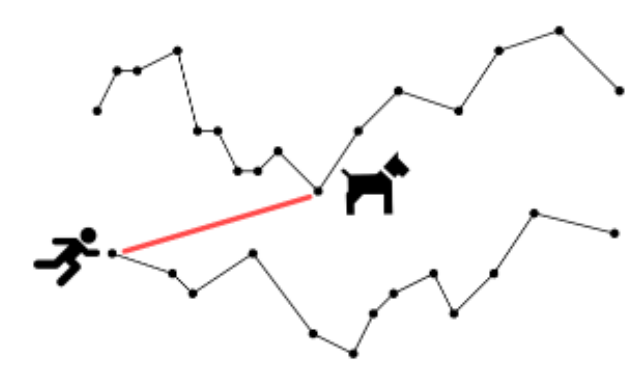
\includegraphics[width=0.5\linewidth]{images/fd.png}
\end{figure}

\paragraph*{Metric indexing principles}
Given a metric dataset $P \subseteq U$, one of the two following principles can be applied to partition it into two subsets: 
\begin{enumerate}
    \item Ball decomposition: take a point $v$, known as vantage point, compute the distances of all other points $p$ with respect to $v$,$ D(p,v)$, and define: 
        \[P_1=\{p|D(p,v)\leq r_v\}\]
        \[P_2= \{p|D(p,v)>r_v\}\]
        Consider a range query ${p|D(p,q)\leq r}$.
        If $D(q,v)>r_v+r$ we can conclude that no point in $P_1$ belongs to the result. 
        Similar arguments apply to $P_2$. 
    \item Generalized hyperplane: take two points $v_1$ and $v_2$, compute the distances of all other points $p$ with respect to $v_1$ and $v_2$, and define: 
        \[P_1=\{p|D(p,v_1)\leq D(p,v_2)\}\]
        \[P_2=\{p|D(p,v_2)<D(p,v_1)}\]
        Consider a range query $\{p|D(p,q)\leq r\}$.
        If $D(q,v_1)-D(q,v_2)>2r$ we can conclude that no point in $P_1$ belongs to the result. 
\end{enumerate}

\subsection{M-tree}
The M-tree has been the first dynamic, paged, and balanced metric index. 
It generalizes R-tree principles to arbitrary metric spaces. 
At a first sight the M-tree looks like an R-tree.
However, the M-tree only knows about distance values, thus it ignores coordinate values and does not rely on any geometric reasoning. 

\paragraph*{Structure}
Recursive bottom-up aggregation of objects based on regions. 
Regions can overlap
Each node (except the root) can contain up to $C_{\text{max}}$ entries, but not less than 
\[C_{\text{min}} \leq 0.5\cdot C_{\text{max}}\]

Each node N of the tree has an associated region, $\text{Reg}(N)$, defined as: 
\[\text{Reg}(N)=\{p|p\in U,D(p,v_N) \leq r_N\}\]
Here, $v_N$ (the “center”) is also called a routing object, and $r_N$ is called the covering radius of the region. 
The set of indexed points $p$ that are reachable from node $N$ are guaranteed to have $D(p,v_N) \leq r_N$. 
This immediately makes it possible to apply the pruning principle: if $D(q,v_N)>r_N+r$ then prune node $N$. 

In leaf nodes an entry $E$ in node $N$ has the form $E=\left\langle \text{ObjFeatures}, \text{distP}, \text{RID} \right\rangle $, where: ObjFeatures are the feature values of the indexed object, and distP is the distance between the object and its parent routing object (i.e, the routing object of node $N$). 
In internal nodes an entry $E$ in node $N$ has the form $E=\left\langle \text{RoutingObjFeatures}, \text{CoveringRadius}, \text{distP}, \text{PID} \right\rangle $, where RoutingObjFeatures are the feature values of the routing object, CoveringRadius is the radius of the region, and distP is the distance between the routing object and its parent routing object (undefined for entries in the root node). 

\paragraph*{Characteristics}
Pre-computed distances distP are exploited during query execution to save distance computations. 
Let $v_P$ be the parent routing object of $v_N$. 
When we consider the entry of $v_N$, we have already computed the distance $D(q,vP)$ between the query and its parent. 
As a result, we know the distance $D(v_P,v_N)$. 
From the triangle inequality we have that: 
\[D(q,vN) \geq \left\lvert  D(q,v_P) - D(v_P,v_N)\right\rvert\]
Thus we can prune node $N$ without computing $D(q,v_N)$ if: 
\[\left\lvert D(q,v_P) - D(v_P,v_N)\right\rvert > r_N + r\]

\paragraph*{Operations}
The procedure to insert a new object is based on a Penalty method. 
The Penalty method considers the increase of the covering radius needed to accommodate the new object. 
For managing a split, there are several alternatives, among which:
\begin{itemize}
    \item \texttt{mM_RAD} minimize the maximum of the two resulting radius. 
    \item \texttt{M_LB_DIST} choose the closest and the farthest object from $v_N$.
\end{itemize}
Experiments demonstrate that \texttt{mM_RAD} is the best. 